\chapter{Results}
This section will present the results of the measurements with ZnTe and GaP as emitter crystals.
Calculations will be made to determine the electricfield strength of the produced $\si{\tera\hertz}$ radiation aswell as the Power of said radiation.
Futher a comparission between the different spectras of ZnTe and GaP will be shown and the efficiency in producing radiation will be discussed.

\section{Zinc telluride}
For this measurments a $\SI{1}{\milli\meter}$ thick ZnTe crystal is used as the emitter.
Another $\SI{1}{\milli\meter}$ thick ZnTe crystal is used as the detector.
The measurements are taken as described in section \ref{sec:execution}.
At this point it should be said, that the Znte crystal that is used as the emitter has two burn marks on it.
The burned crystal can be seen in figure \ref{fig:ZnTe_burned}.
Obviously the burned part of the crystal negatively effects the efficiency of $\si{\tera\hertz}$ production.
Which is why the part of the laser with the highest power is not focused on the burned part.
Still some of the laser hits the burned part of the crystal.
\\\\
To develop an understanding for the data the first figure that should be looked at is the time resolved EOS data.
For this the lock-in Amplifier output is plotted against the time delay between pump and probe beam.
The figure \ref{ZnTe:2_11_30_signal} shows the resulting plot.
This measurement is taken with a pump power of $\SI{135.0}{\milli\W}$, which is the highest pump power that is used.
The typicall trend of a $\si{\tera\hertz}$ pulse can clearly be seen.
Befor the pulse starts the signal is balanced at $X(V)=0$.
\begin{figure}
    \centering
    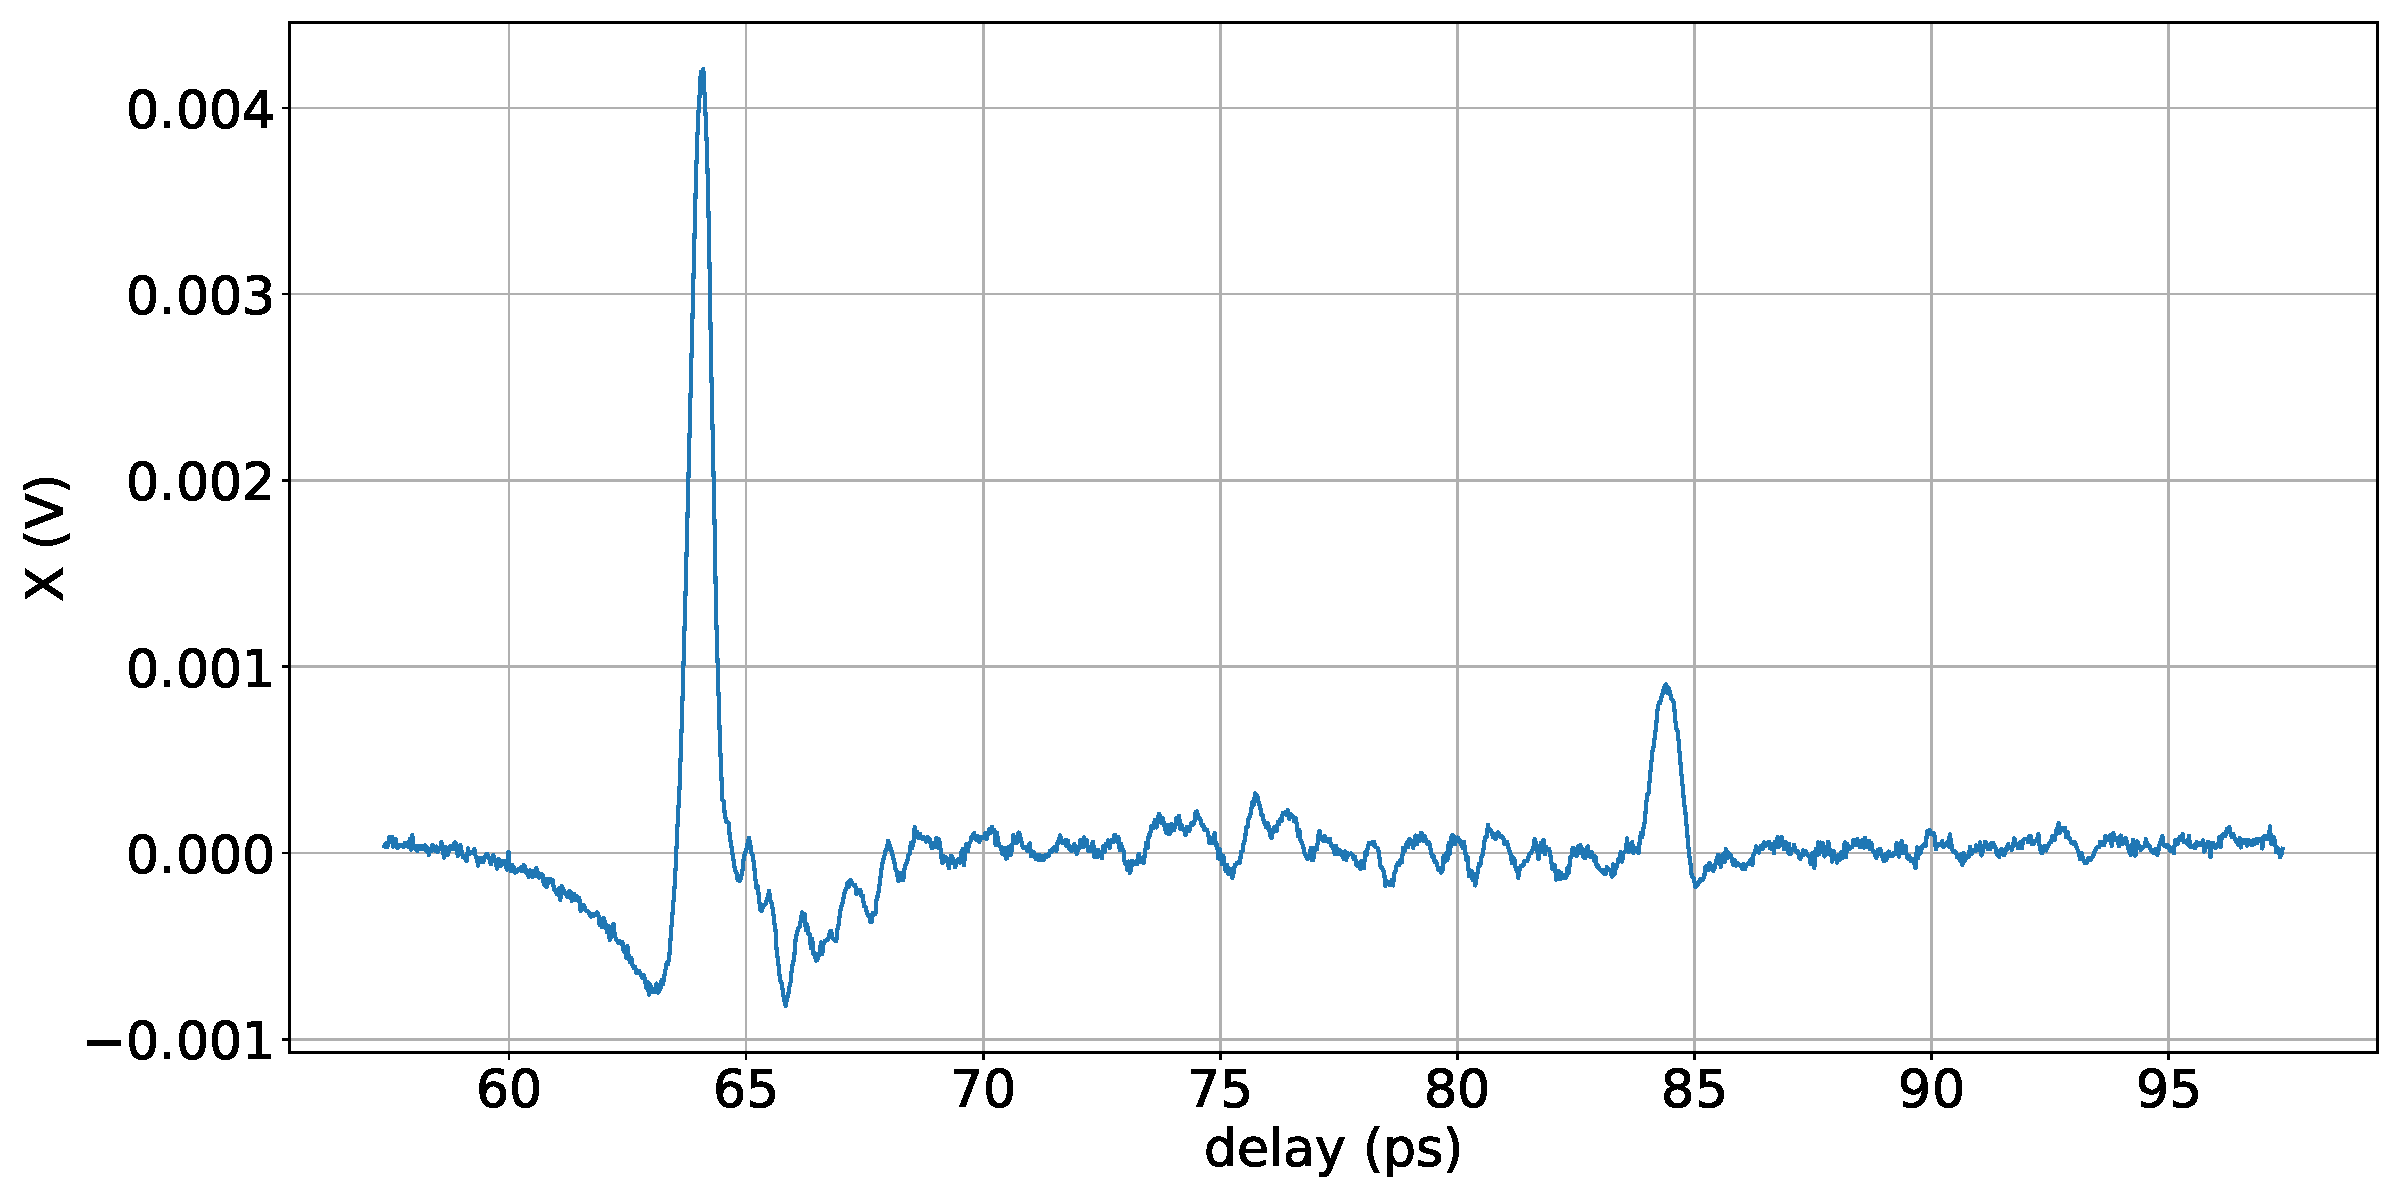
\includegraphics[width=0.75\textwidth]{Plots/2_11_30_20normalX.pdf}
    \caption{The $\si{\tera\hertz}$ pulse, that is measured by EOS, with a pump power of $\SI{135.0}{\milli\W}$.
    The EOS signal is plotted against the delay in $\si{\pico\second}$.
    A post pulse can be seen at a delay of $\SI{84}{\pico\second}$.}
    \label{ZnTe:2_11_30_20_signal}
\end{figure}
\\
At a delay of about $\SI{58}{\pico\second}$ the pulse starts, which manifests in a an increasingly negativ $X(V)$ value.
After about $\SI{5}{\pico\second}$ after the start the minimum is reached and the lock-in Amplifier output increases drastically up to a value of $\SI{4.20669}{\milli\V}$.
Here the maximum of the plot is reached, which corresponses to the maximum $\si{\tera\hertz}$ electricfield strength inside the detector crystal.
After the maximum the signal drops almost to zero.
\\
From this point on there are some oszillations, but no major features are visible. %are those oszialltions acuatlly caused by water?
Up until a delay of $\SI{84}{\pico\second}$, where the post pulse starts.
The post pulse is caused by reflections of the $\si{\tera\hertz}$ pulse inside the crystal.
Which is why the post pulse is just an echo of the intial pulse and thus alters the signal in a negativ way.
For futher calculations the data that is taken up until the post pulse will be used.
\\\\
\FloatBarrier
To confirm that the pulse that is shown in figure \ref{ZnTe:2_11_30_20_signal} actually corresponses to a $\si{\tera\hertz}$ pulse a Fourier-Transformation of the data is calculated. %Do I need to mention FFT in theory?
Because the Fourier-Transformation is done numerically the FFT function of the python package scipy \cite{scipy} is used.
The resulting Fourierspectrum is shown in figure \ref{fig:2_11_30_20_fft}.
The Spectrum is also plotted against a logarithmic x-axis, which gives the plot in figure \ref{fig:2_11_30_20_fft_log}.
With this it is easy to confirm that the produced radiation actually lies in the $\si{\tera\hertz}$ regime.
Most of the radiation that is produced has a frequenzy between $0.3-1.1\,\si{\tera\hertz}$, but radiation with even higher $\si{\tera\hertz}$ frequencies is produced aswell.
Espacially in the spectrum which is plotted against the logarithmic x-axis the water absorption line of $\SI{1.226}{\tera\hertz}$ is clearly visible.
This is due to the water vapor in the air between emmitter and detector crystal.
Some absorption lines at even higher frequencies are visible too.
\begin{figure}%
    \centering
    \caption{The Fourierspectrum of the data, that is collected with the highest pump power of $\SI{135.0}{\milli\W}$.
    One of the spectras is plotted against a logarithmic axis to see the higher frequencies aswell.}%
    \begin{subfigure}{0.35\textwidth}%
        \centering%
        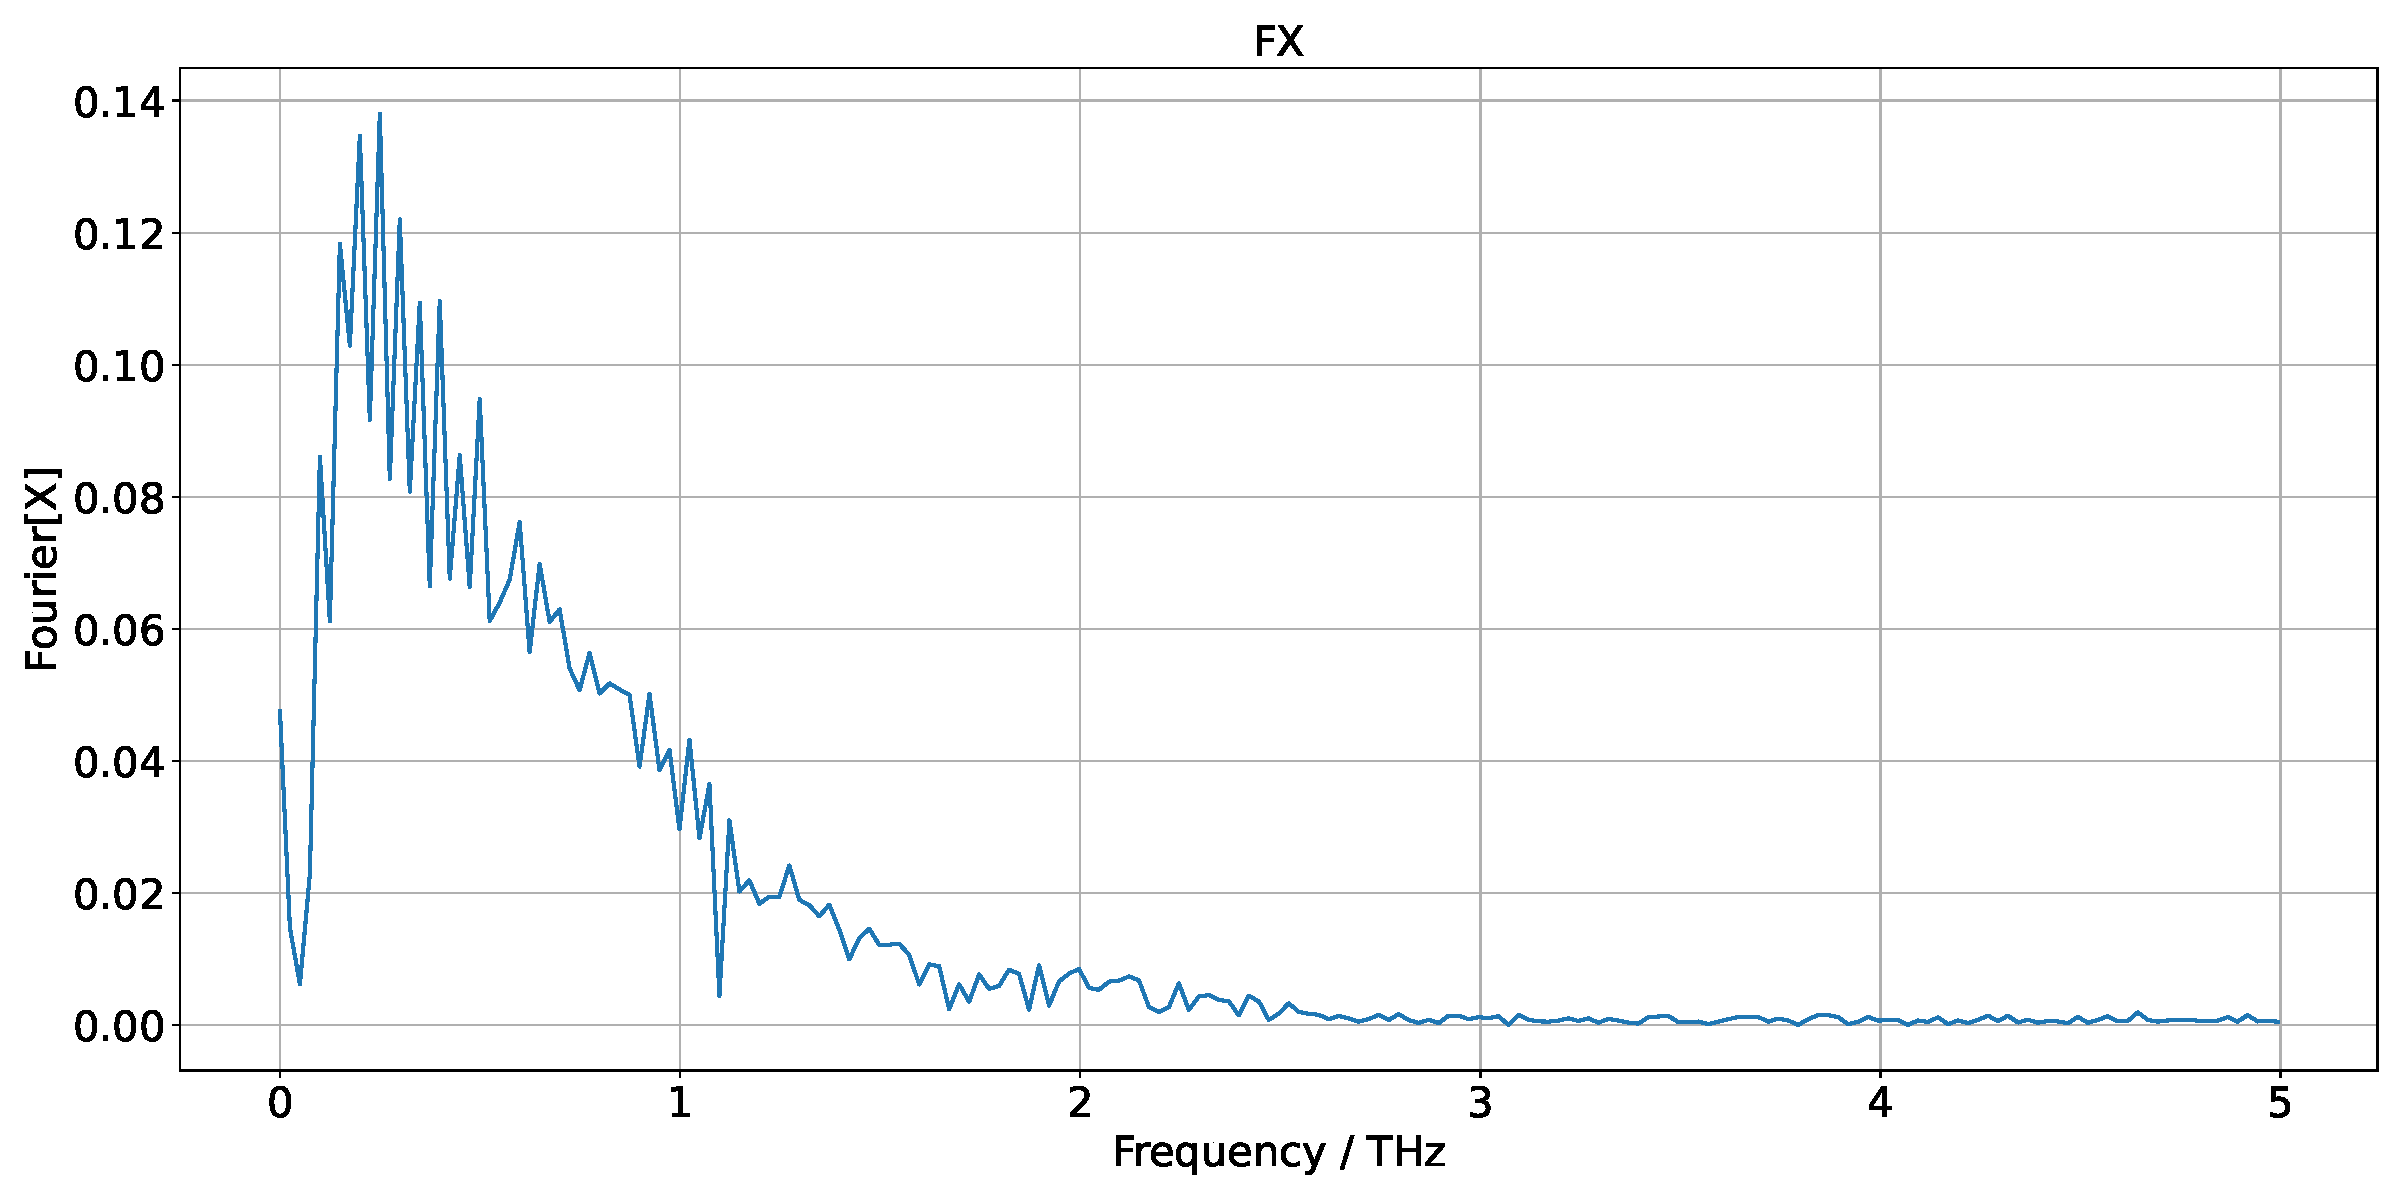
\includegraphics[height=3.5cm]{Plots/2_11_30_20normalFX.pdf}%
        \caption{The Fourier-Transformation of the $\si{\tera\hertz}$ pulse shown in figure \ref{ZnTe:2_11_30_20_signal}.
        It can clearly be seen that the frequency of the radiation lies in the lower $\si{\tera\hertz}$ regime.}%
        \label{fig:2_11_30_20_fft}%
        \end{subfigure}%
    \hfill% Fills available space in the center -> space between figures
        \begin{subfigure}{0.35\textwidth}%
        \centering%
        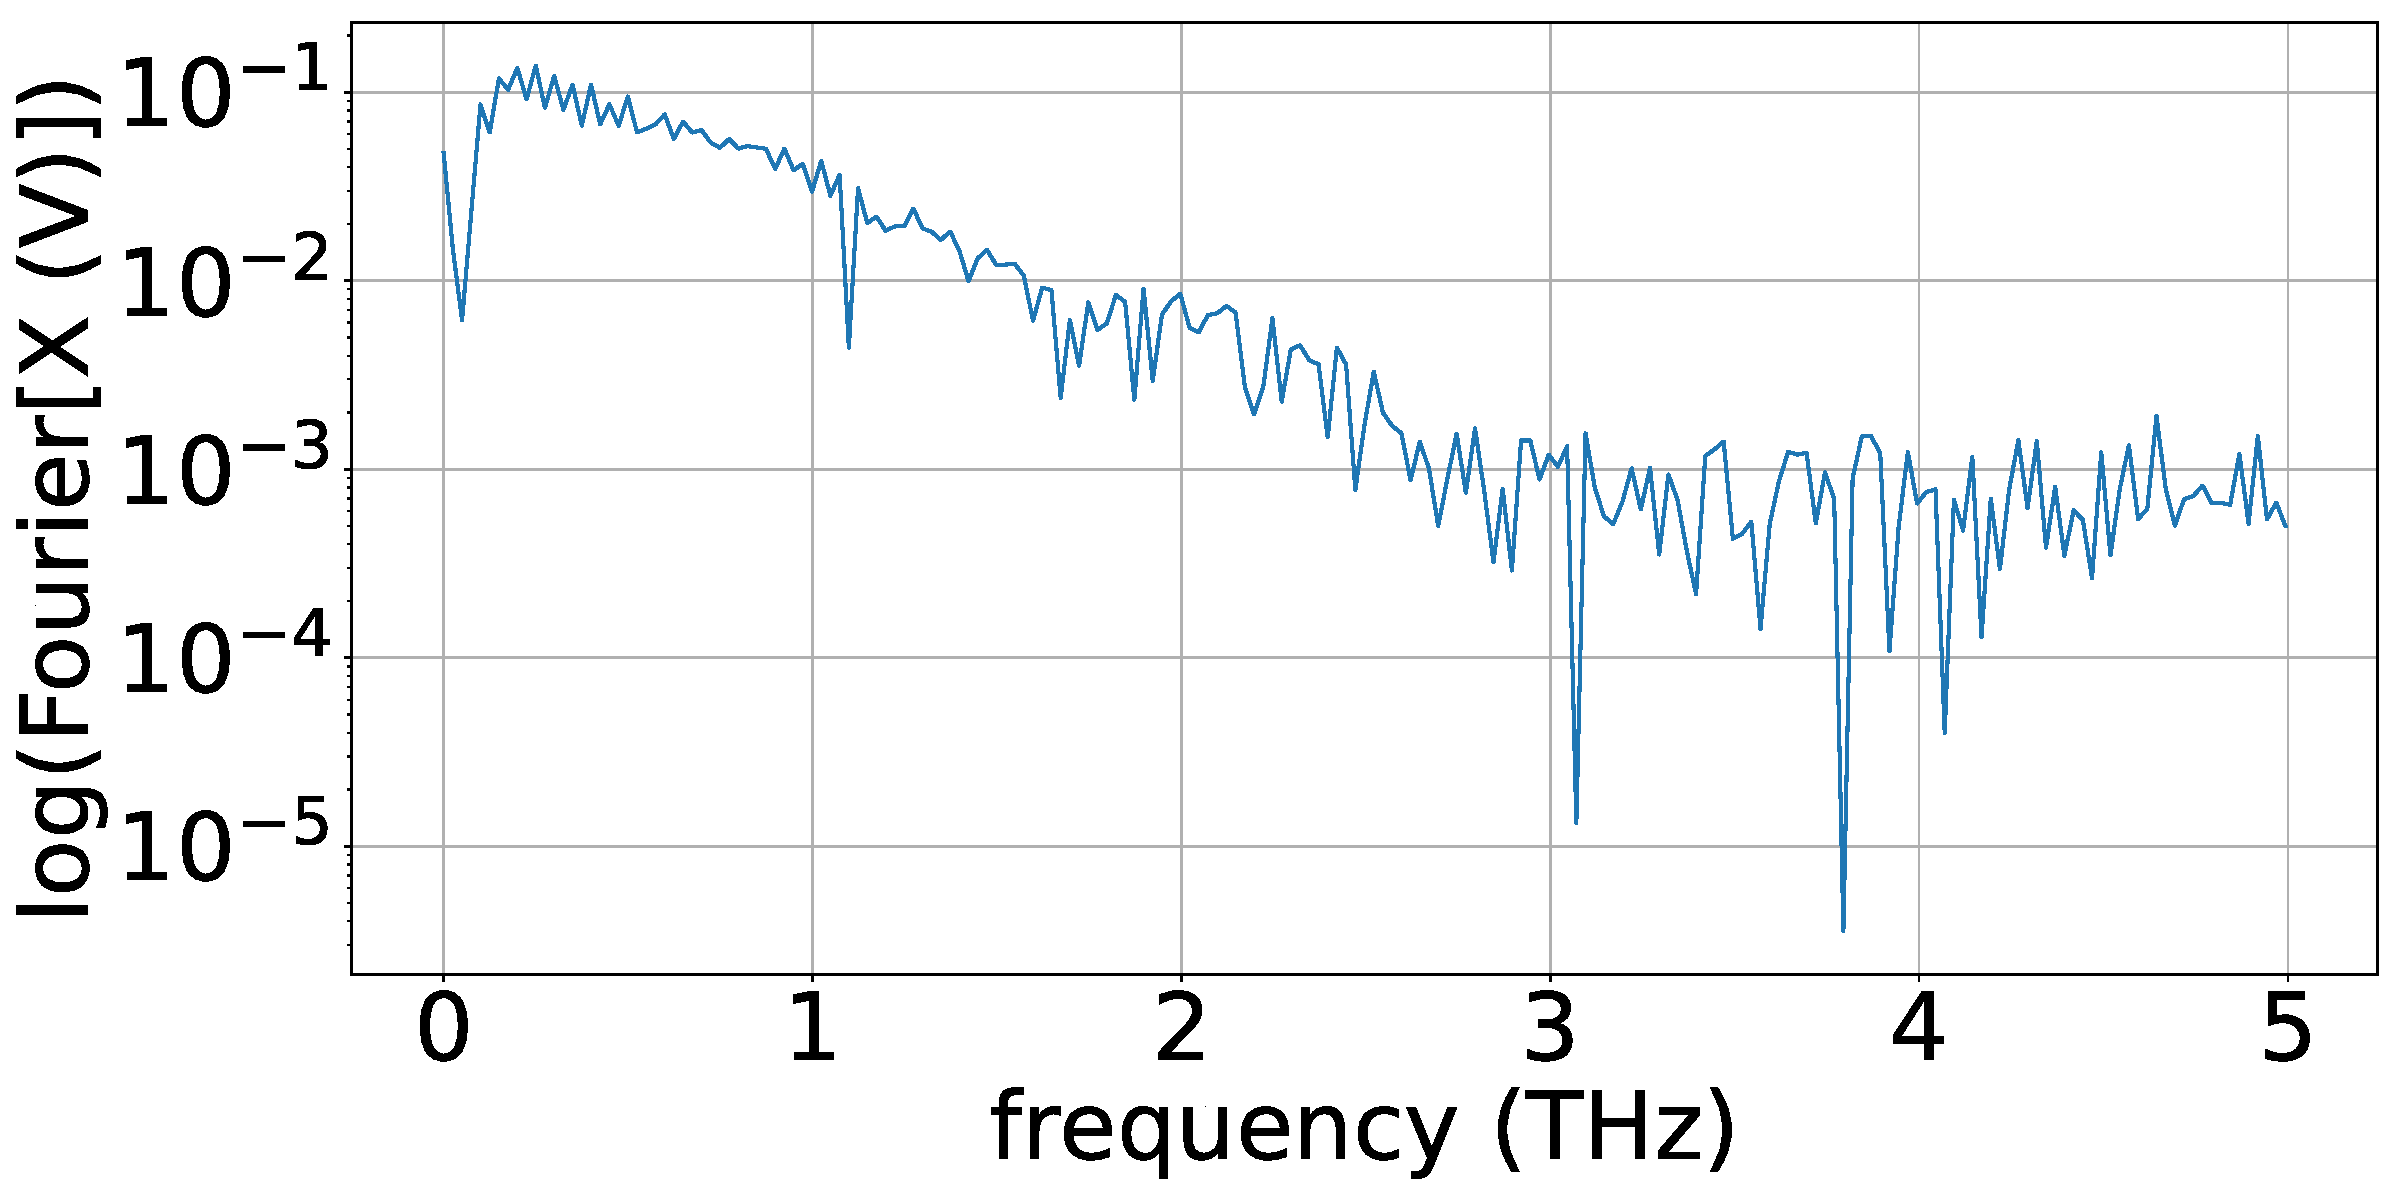
\includegraphics[height=3.5cm]{Plots/2_11_30_20normallog(FX).pdf}%
        \caption{The Fourierspectrum of the data shown in figure \ref{ZnTe:2_11_30_20_signal} plotted against a logarithmic x-axis.
        This shows that higher $\si{\tera\hertz}$ frequencies are produced aswell. Some absorption lines can also bee seen.}%
        \label{fig:2_11_30_20_fft_log}%
    \end{subfigure}%
    \label{fig:fourier_znte}%
\end{figure}%
\FloatBarrier

\subsection{Fluence measurments}

\subsection{Electric field measurments}
To determine the peak electricfield of the  $\si{\tera\hertz}$ pulse, several measurements of $A$, $B$ and $A-B$ are taken as described in section \ref{sec:field}.
To get the best result and minimize the error through noise for $A$ and $B$, their value is measured $500$ times.
After the data is taken their mean value is used for futher calculations with error being the standard deviation.
All futher errors are calculated by 
With those the electricfield is calculated by equation \ref{eq:electricfield_A_B}.



\section{Gallium phosphide}
\subsection{Fluence measurments}
\subsection{Electric field measurments}


\section{Comparisson}